\section{HTML5}

Für die Implementierung der Browseranwendung wird auf den aktuellen Entwurf des  zukünfitgen HTML5
Standards zurückgegriffen. 

\acr{html} ist eine Sprache, die der strukturierten Beschreibung von Webseiten dient. Die Sprache
wurde in ihrer ursprünglichen Form  von 1989-1992, lange vor dem sogenannten Web 2.0, von
Wissenschaftlern des Europäischen Kernforschungsinstitut CERN entwickelt. Sie war der erste nicht
proprietäre globale Standard zur digitalen Übertragung von strukturierten  Dokumenten. Die Sprache
\acr{html} allein ist nicht geeignet, um dynamische Inhalte  wie sie heute praktisch auf allen
modernen Webseiten vorkommen, zu beschreiben. 

Der heutige HTML5-Standard geht weit über die Sprache \acr{html} selbst hinaus und  umfasst vor
allem auch die Scriptsprache \acr{js} und die darin verfügbaren Bibliotheken sowie das \acr{dom},
auf das in  Scripten zugegriffen werden kann, um den angezeigten Inhalt dynamisch zu verändern.
\cite{html5}

\subsection{Dokumenobjektmodell}

Das \textit{\acr{dom}} ist eine Schnittstelle, die es erlaubt \acr{html}- bzw. \acr{xml}-Dokumente zu
modifizieren und bildet damit die Grundlage für die Realisierung dynamischer Webseiten.

Der Einstiegstpunkt in das \acr{dom} ist der \texttt{document}-Knoten, welcher in \acr{js}
global verfügbar ist und von welchem aus die gesamte Baumstruktur erreichbar ist. Jeder
\acr{html}-Tag, jedes Attribut und jeder Text wird als ein Objekt, bzw. ein Knoten im Baum
repräsentiert. Über verschiedene Methoden ist es möglich die Kinder-, Geschwister- und Elternknoten
zu erhalten. Durch funktionen wie \texttt{appendChild} ist es schließlich möglich, neue Elemente
in das \acr{dom} zu integrieren bzw. bestehende zu modifizieren. \cite{dom}

\subsection{Cascading Styles Sheets}

\acr{css} ist eine Sprache, die der Definition von  Stilen bzw. Stilvorlagen für die Anzeige von
Webinhalten dient.

Durch die Trennung von \acr{html} und \acr{css} wird erreicht, dass \acr{html}-Dokumente sich auf
den Inhalt einer Seite beschränken, während alle die grafische Anzeige  belangenden Aspekte in die
Stilvorlagen in \acr{css}-Dateien ausgelagert  werden.

\subsubsection{CSS3}
\label{sec:css3}

In der kommenden \acr{css} Version 3.0, die bereits zu großen Teilen von den meisten aktuellen
Browsern unterstützt wird, kommen einige interesante Neuerungen hinzu, die es vor allem ermöglichen,
Anwendungen, welche man Bisher in Frameworks wie \textit{Flash} oder \textit{Silverlight}
implementiert hat nun in reinem \acr{html}+\acr{css} zu verwirklichen. Die für die Realisierung der
browserbasierten Entwicklungsumgebung relevanten Neuerungen umfassen im speziellen:

\begin{itemize}
  \item Einbetten von Schriftarten,
  \item Animationen und Übergänge,
  \item Verhindern von Textmarkierungen und
  \item Festlegen der Sichtbarkeit von Elementen für den Mauszeiger.
\end{itemize}

\subsubsection{LESS}

\label{sec:less}

Auch \acr{css}3 hat immernoch einige konzeptionelle Einschränkungen, welche die Benutzung
erschweren:

\begin{itemize} 
  \item Es ist nicht möglich Variablen zu definieren, um Werte, die an
vielen Stellen vorkommen nur einmal definieren zu müssen. 
  \item Es fehlen Funktionsdefinitonen, um ähnliche
oder abhängige Definitionen  zusammenzufassen und zu parametrisieren. 
  \item Die Hierarchie einer
\acr{css}-Datei ist flach, obwohl die Definitionen geschachtelt sind. Dies reduziert die Lesbarkeit
der Dateien. 
  \item Wenn aus Gründen der Übersichtlichkeit \acr{css}-Definitionen in mehrere Dateien aufgeteilt
werden, müssen alle Dateien einzeln geladen werden, was zu längeren Ladezeiten führt. \end{itemize}

\textit{LESS} ist eine Erweiterung von \acr{css}, die unter anderem  Variablen- und
Funktionsdefinitionen, verschachtelte Definitionen sowie  Dateiimports erlaubt. Damit werden die
oben genannten Einschränkungen von \acr{css} zu großen Teilen aufgehoben.

Das Play Framework (Siehe Abschnitt\,\ref{sec:play}) ermöglicht es, die Stylesheet-Sprache
LESS zu verwenden, ohne dass diese auf Browserseite unterstützt werden muss. Hierfür
werden die in  LESS definierten Stylesheet auf Serverseite in CSS übersetzt  und
dem Browser zur Verfügung gestellt. Dafür müssen die Dateien an einem vorher konfigurierten Ort
liegen. Nach der Übersetzung werden sie an derselben Stelle zur Verfügung gestellt wie normale
CSS-Dateien.

\subsection{JavaScript}

\textit{JavaScript} ist eine dynamisch typisierte, klassenlose, objektorientierte Scriptsprache, die
aktuell der Standard in der Entwicklung von clientseitigem Code für dynamische Webinhalte ist. Der
Kern von \acr{js} wurde von der \textit{Ecma International} als \textit{ECMAScript} normiert. Durch
\acr{js} ist es möglich Webseiten dynamisch zu verändern. Für eine gute Einführung in die Konzepte
von \acr{js} sei an dieser Stelle auf \cite{js} verwiesen.

\subsubsection{CoffeeScript}
\label{sec:coffeescript}

JavaScript wurde in Eile entwickelt und normiert, da zur Zeit der Entstehung ein schneller Bedarf an
einer normierten Sprache für das Web bestand. Dadurch sind jedoch auch einige Unschönheiten in den
Sprachkern gedrungen. So ist beispielsweise die C-artige Syntax für eine eher funktional angehauchte
Sprache wie \acr{js} ungeeignet, da Funktionsdefinitonen durch geschweifte Klammern, das
Schlüsselwort \texttt{function} und ein \texttt{return} Statement unnötig aufgeblasen werden und
damit unleserlicheren Code erzeugen. Darüber hinaus fehlt in \acr{js} jede Möglichkeit der
Modularisierung. Da noch nicht einmal Klassen existieren, führt das bei reinem JavaScript schnell zu
unwartbarem Code. Ein weiterer Stolperstein ist das Schlüsselwort \texttt{this}, das nicht immer
klar zu verstehen ist, da es in Funktionsaufrufen seine Bedeutung wechseln kann.

\textit{CoffeeScript}\footnote{http://www.coffeescript.org} ist eine neue Scriptsprache mit dem Ziel
diese \glqq Problemzonen\grqq von \acr{js} auszumerzen. CoffeeScript hat eine eher an funktionale
Sprachen wie Haskell erinnernde Syntax mit Verschachtelungen über Whitespace und einem
\texttt{->}-Operator zur Funktionsdefinition. Darüber hinaus bietet CoffeScript die Möglichkeit
Klassen zu definieren und führt das Konzept der Vererbung ein. Das \texttt{this}-Schlüsselwort kann
an Instanzen von Klassen gebunden werden. CoffeeScript Dateien werden zu optimiertem \acr{js} Code
kompiliert, der den Vorgaben des \textit{\acr{js}
Linter}\footnote{http://www.javascriptlint.com/} entspricht. Im Einzelnen sind die Verbesserungen
gegenüber \acr{js}:

\begin{itemize}
  \item Vereinfachte Syntax für Funktionsdefinitionen, Arrays, Blöcke,
  \item automatisches Initialisieren von Variablen (\textit{lexical scoping}),
  \item variable Parameterlisten (\textit{splats}),
  \item universellere Iterationsschleifen (\texttt{for}),
  \item vereinfachtes \textit{slicing} und \textit{splicing} (Arrayoperationen),
  \item Ausdrucksorientiertheit,
  \item Klassen und Vererbung,
  \item ein Existenzoperator,
  \item destrukturierende Zuweisungen (z.B. \texttt{[a,b] = [c,d]}),
  \item Bindung von \texttt{this} an Klasseninstanzen sowie
  \item mehrzeilige Strings und reguläre Ausdrücke mit Kommentaren.
\end{itemize}

Genauso wie für LESS existiert im Play Framework (Siehe Abschnitt\,\ref{sec:play}) eine serverseitige
Unterstützung  für CoffeeScript. Die in CoffeeScript geschriebenen Dateien  werden ebenfalls an
gleicher Stelle wie normale \acr{js}-Dateien dem  Browser als \acr{js} zur Verfügung gestellt.

\subsection{HTTP}

Das \acr{http} ist das im Intenet verwendete Standardprotokoll zur Übertragung von Daten. (Siehe
auch \cite{http}) Leider ist \acr{http} für die Implementierung von hochdynamischen Webapplikationen
nur bedingt geeignet, da Anfragen immer vom Browser gestellt werden, aber keine Möglichkeit
vorgesehen ist, in die andere Richtung initiativ zu kommunizieren.  Auf Grund der Einschränkungen
des Protokolls, kam es in der Vergangenheit zur Entwicklung einiger Tricks um die sogenannten
\textit{Server-Pushes} zu realisieren. Die bekanntesten sind das \textit{Polling}, bei dem in
kleinen Abständen Anfragen an den Server gestellt werden, und \textit{Comet} welches auf verzögerten
Antworten vom Server basiert. Beide Lösungen werfen neue Probleme auf. Zum einen eine deutlich
erhöhte Nutzung von Verbindungskapazitäten beim Polling und zum anderen das häufig vollständige
Ausbleiben von Serverantworten und damit die fehlende Freigabe von Threads bei Comet-Anfragen.

\subsubsection{AJAX}

\acr{ajax} ist keine Bibliothek und auch kein  Standard sondern ein Konzept zur Übertragung von
Daten  zwischen Browser und Webserver per \acr{http} auf dynamischen Webseiten. Hierbei wird das
\acr{js}-Objekt \texttt{XMLHttpRequest} verwendet, um während der Anzeige einer Webseite, Daten vom
Server nachzuladen bzw. dem Server Daten zu senden, ohne dass die Webseite neu geladen werden muss
wie es bei klassischen Webseiten der Fall war. Ursprünglich und namensgebend wurde für die
Übertragung der Daten XML verwendet. Mittlerweile ist es nach dem abgflauen des XML-Hypes wegen der
guten Untersützung in \acr{js} und den meisten Webframeworks auch üblich \acr{json} zur Übertragung
zu nutzen. \cite{ajax}

\begin{figure}[ht]
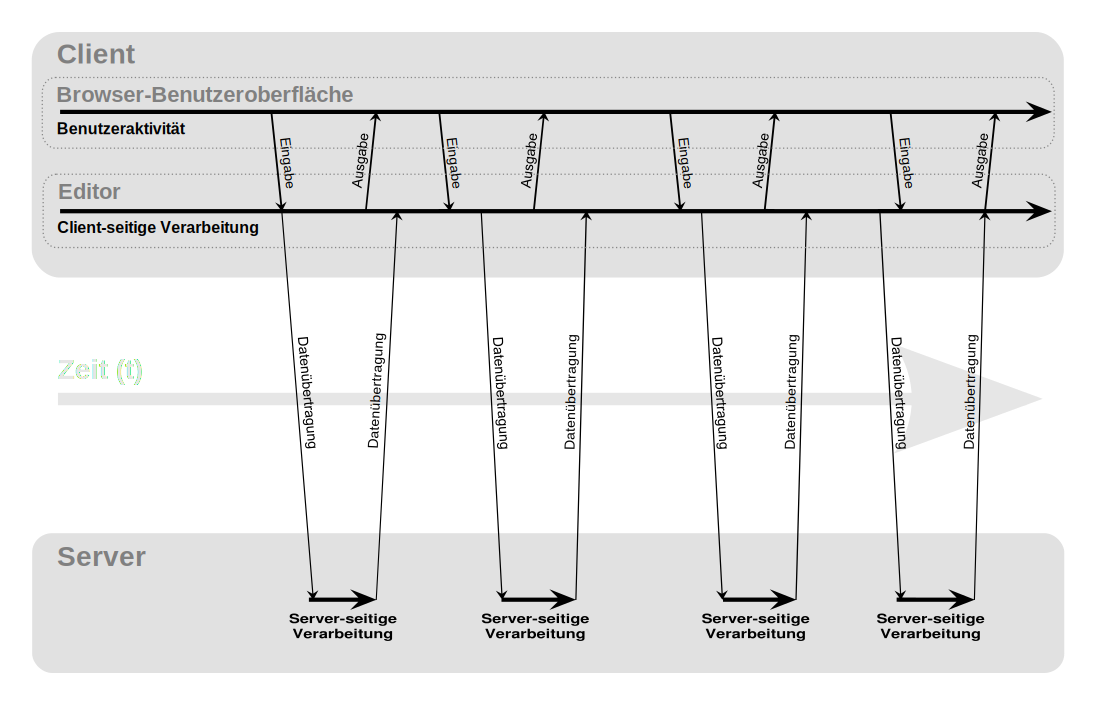
\includegraphics[width=\linewidth]{images/diagram-ajax}
  \caption{Ajax Modell einer Web-Anwendung (asynchrone Datenübertragung)}
  \captionsetup{font={footnotesize,bf,it}}
  \caption*{Quelle: Wikipedia}
  \label{fig:diagram-ajax}
\end{figure}

\subsection{WebSockets}

WebSockets sind ein in HTML5 neu eingeführter Standard zur bidirektionalen  Kommunikation zwischen
Browser und Webserver. Hierbei wird anders als bei  AJAX eine direkte TCP-Verbindung hergestellt.
Diese Verbindung kann sowohl von  Browser-, als auch von Serverseite aus gleichartig verwendet
werden. Das macht es  unnötig, wie bei AJAX wiederholte Anfragen oder Anfragen ohne Zeitbegrenzung
zu  stellen, um Informationen vom Server zu erhalten, wenn diese verfügbar werden. Ein weiterer
Vorteil gegenüber HTTP-Anfragen ist, dass durch die direkte permanente Verbindung kein
Nachrichtenkopf mehr nötig ist. Das macht es deutlich  effizienter, viele kleine Nachrichten zu
versenden.

Zum Aufbau einer WebSocket Verbindung wird einmalig zu Beginn eine \acr{http} Anfrage vom Browser
gestellt, die der Server dann im Erfolgsfall mit der Eröffnung des WebSockets beantwortet.
\cite{websockets}

\clearpage

\subsection{JavaScript-Bibliotheken}

Über den HTML5 Standard hinaus werden für die Strukturierung der Anwendung einige
\acr{js}-Bibliotheken benötigt, die im Folgenden kurz erläutert werden.

\subsubsection{jQuery}

Die Bibliothek \textit{jQuery}\footnote{http://www.jquery.com} ist heute ein defacto-Standard in der
Webentwicklung. In erster Linie erleichtert es den Zugriff und die Manipulation des \acr{dom},
bietet aber darüber hinaus zahlreiche Vereinfachungen im Umgang mit alltäglichen Aufgaben der
Webentwickling. Besonders erwähnenswert ist hierbei auch die \acr{ajax}-Abstraktion. Eine gute
Einführung in jQuery bietet \cite{jquery}.

\subsubsection{Backbone und Underscore}

\textit{Backbone}\footnote{backbonejs.org} ist eine Bibliothek, die der Strukturierung von
sogenannten \textit{single-page}-\acr{js}-Anwendungen dient. Backbone baut auf der allgemeinen
\textit{Underscore}\footnote{underscorejs.org}-Bibliothek auf, die einige Erleicherungen im Umgang
mit Daten in \acr{js} bietet.. Backbone führt das Model-View-Controller Konzept in
Browseranwendungen ein und bietet hierfür einige Prototypen, von denen abgeleitet werden kann um
eigene Modelle und Views zu implementieren, die dann über Events deklarativ miteinander verküpft
werden können.

Besonders interessant ist die Möglichkeit, die im \acr{html}5 Standard neu eingeführte
\textit{History API} in Backbone zur Navigation zu verwenden. Dadurch ist es möglich in einer
\acr{js}-Anwendung, welche die Seite nicht neu aufbaut, sondern immer nur Teile verändert,
Navigation einzuführen, sodass der Benutzer zwischen den Zuständen Navigieren kann. Hierfür bietet
Backbone die sogenannten \texttt{Router} in denen von URLs auf Zustände der Anwendung und umgekehrt
abgebildet werden kann. Eine gute Einführung in die Bibliothek findet sich in \cite{backbone}.

\subsubsection{RequireJS}
\label{sec:requirejs}

Da JavaScript von Haus aus keine Möglichkeit der Modularisierung bietet, komplexe Anwendungen
jedoch ohne Modularisierung kaum wartbar bleiben, haben sich unterschiedliche Lösungsansätze für
dieses Problem entwickelt. Einer der  umfassendsten ist die Bibliothek \textit{RequireJS}.

Mit der Funktion \texttt{define} können Module in Form von Funktionsdefinitionen  definiert werden.
Alle lokalen Variablen in dem Modul sind anders als bei  normalen Scripten außerhalb nicht mehr
sichtbar, da sie innerhalb einer  Funktion definiert wurden. Das Funktionsergebnis ist das was nach
außen sichtbar  ist. Dies kann ein beliebiges Objekt (also auch eine Funktion) sein.

Die so definierten Module können Abhängigkeiten untereinander spezifizieren,  indem der
\texttt{define}-Funktion eine Liste von Modulen übergeben wird, die  das aktuelle Modul benötigt.
Die \textit{RequireJS}-Bibliothek sorgt dann dafür,  dass diese Module geladen werden bevor das
aktuelle Modul ausgeführt wird.

RequireJS erlaubt es, den  \acr{js}-Code für den Produktiveinsatz zu optimieren. Dafür
gibt es  das sogenannte \textit{r.js}-Script, das unter anderm alle Abhängigkeiten in eine Datei
zusammenfasst und den Code durch entfernen von Whitespaces und Kommentaren  sowie umbenennen
von Variablennamen verkürzt. Zur Entwicklungszeit ist dieser nicht mehr lesbare Code nicht
erwünscht. Deswegen bietet das Play Framework (Siehe Abschnitt\,\ref{sec:play}) eine integrierte
Version von RequireJS, die automatisch den lesbaren Code zur Entwicklungszeit  bereitstellt, im
Produktiveisatz jedoch den optimierten.